\documentclass[a4paper,cs4size]{BHCexam}
%\documentclass[a4paper,cs4size,answers]{BHCexam}

\usepackage{multicol} % 分栏
\pagestyle{fancy}
\fancyfoot[C]{\kaishu \small 第 \thepage 页 共 \pageref{lastpage} 页}
%\fancyhead[L]{\includegraphics[width=2cm]{qrcode.png}}
\title{质量密度习题课}
%\subtitle{数学文科试卷}
%\notice{满分150分, 120分钟完成, \\	允许使用计算器,答案一律写在答题纸上.}
%\author{Gavin Chen}
%\date{\today}

\begin{document}
\maketitle
\begin{groups}
    \group{}{}
    \zihao{-4}
    \begin{questions}[]

        \question[5] 质量为$7.8kg$的铁球,其体积是$2\times 10^{-3}m^3$。忽略空心部分的质
        量。已知铁的密度为$7.8\times 10^3 kg/m^3$。求:
        \begin{subquestions}
            \subquestion 空心部分的体积;
            \subquestion 若在空心部分注满水后球的总质量。
        \end{subquestions}

        \begin{solution}{0.5cm}
            \methodonly 略
        \end{solution}

        \vspace{5cm}
        \question[5] 体积和质量都相等的空心铝球、铜球和铁球($\rho_{\text{铜}}>\rho_{\text{铁}}>\rho_{\text{铝}}$),空心部分的质
        量忽略不计。将空心部分注满水后(\quad\quad\quad)。
        \fourchoices{铝球质量最大}
        {铁球质量最大}
		{铜球质量最大}
		{三个球质量一样}
        \vspace{1cm}

        \question[5] 有一质量为$0.12kg$的圆柱体空玻璃瓶,按如图所示方式放置在水平桌面上,它的底面积为$2.94\times 10^{-3}m^2$,当瓶内装满水时,瓶和水的总质量为$0.45kg$,求:
        \begin{subquestions}
            \subquestion 玻璃瓶内水的体积;
            \subquestion 装满水后玻璃瓶对水平桌面的压强;
            \subquestion 在此空瓶中装入一些金属颗粒,测得瓶和金属颗粒的总质量为$0.51kg$。若再在这个瓶中装满水,此时瓶、金属颗粒和水的总质量为$0.79kg$,求金属颗粒的密度。
        \end{subquestions}
        \begin{figure}[htb]
            \flushright
            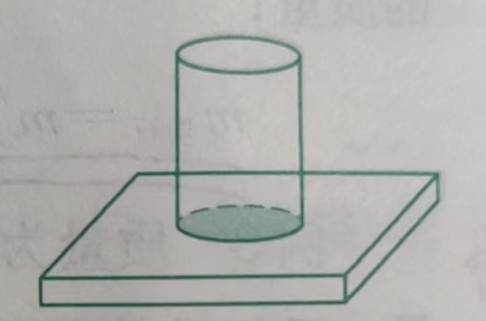
\includegraphics [scale=0.4,trim=0 0 0 0]{./image/physics_mass_1.PNG}
            % \caption{图名}
            \label{fig:fig_mass_1}
        \end{figure}
        \vspace{6.5cm}

        \question[5] 如图所示,两高度均为$h$的桂形容器甲、乙放置在水平地面上,已知甲、乙的底面积分别为$2S$、$S$。甲容器中装满$3\times 10^{-2}m^3$的水。
        \begin{subquestions}
            \subquestion 求甲容器中水的质量;
            \subquestion 往乙容器中注入密度为$\rho_0$的液体,则最多能注入的液体体积为多少?
            \subquestion 将体积为$1\times 10^{-3}m^3$的物体$A$浸没于装满水的甲容器中,将体积为$2\times 10^{-3}m^3$的物体$B$浸没于装满密度为$\rho_0$的液体的乙容器中。
            已知乙容器中溢出液体的质量是甲容器中溢出水的质量的$3$倍。求密度$\rho_0$的大小。
        \end{subquestions}
        \begin{figure}[htb]
            \flushright
            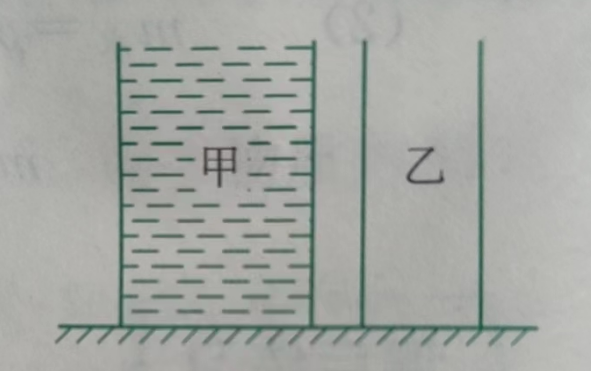
\includegraphics [scale=0.4,trim=0 0 0 0]{./image/physics_mass_2.PNG}
            % \caption{图名}
            \label{fig:fig_mass_2}
        \end{figure}
        \vspace{6.5cm}

        \question[5] 分别计算下面几种情况的密度。
        \begin{subquestions}
            \subquestion 两种物质的密度分别为$\rho_1,\rho_2$,体积分别为$V_1,V_2$,将它们混合在一起,密度为多少?(混合物的体积等于混合物中各物质体积之和)
            \subquestion 两种物质的密度分别为$\rho_1,\rho_2$,将它们等体积混合,混合物的密度为多少?
            \subquestion 两种物质的密度分别为$\rho_1,\rho_2$,将它们等质量混合,混合物的密度为多少?
        \end{subquestions}
        \vspace{6.5cm}

        \question[5] 用盐水选种,要求盐水的密度为$1.1\times 10^3 kg/m^3$。现配制了$0.5dm^3$
        的盐水,称出其质量为$0.6kg$。
        \begin{subquestions}
            \subquestion 配制的盐水是否符合要求?
            \subquestion 若不符合要求,应加盐还是加水?
            \subquestion 应加盐或加水多少?
        \end{subquestions}
        \vspace{6.5cm}

        \question[5] 有一件用金铜合金制成的工艺品,用天平测得它的质量是$600g$,用量筒和水配合测得它的体积是$50cm^3$。
        已知金的密度是$19.3\times 10^3 kg/m^3$,铜的密度是$8.9\times 10^3 kg/m^3$。计算该工艺品的含金量(含金量是指工艺品中金的质量占总质量的百分比)。
        \vspace{6.5cm}

        \question[5] 某工厂用密度为$\rho_1$和$\rho_2$的两种纯金属混合熔炼合金材料。
        若采取$3:2$的比例配方,即密度为$\rho_1$的金属质量取$3$份,密度为$\rho_2$的金属质量取$2$份,那么混合后所得合金材料的密度是多少?



    \end{questions}





\end{groups}


\label{lastpage}
\end{document}
